\chapter{Physical aspects of Fluid-Structure Interaction problems}
\label{cha:physics}


Dynamic models of solids or fluids aim at describing the evolution of an initial configuration through time. Structural mechanics and fluid dynamics use different perspectives when describing the motion of respectively a solid or a fluid particle. When dealing with FSI problems the two approaches need to be combined in order to obtain a suitable description of the two domains and their interface: this aspect is treated in \ref{sec:desc-motion}.

As outlined in the introduction, the fluid and the solid domain of a FSI problem might be described by means of many different models: some of them are outlined in section \ref{sec:models}.  \textit{Dimensional analysis} and the use of dimensionless numbers is a powerful tool used to classify fluid dynamics problems: some of the principles used there can be applied to FSI problems in order to classify them: this can help define and classify FSI problems, as described in section \ref{sec:classification}.

\section{Description of motion}
\label{sec:desc-motion}

In a FSI model, the fluid in motion deforms the solid because of the forces exerted to the structure. The change in the shape of the solid modifies the fluid domain, causing a different flow behavior. For this reason it is necessary to describe formally the kinematics and the dynamics of the whole process. Classical continuum mechanics considers the motion of particles by means of two different perspectives  \cite{batra2006elements}: the \textit{Eulerian description}, briefly described in section \ref{subsec:euler}, and the \textit{Lagrangian description}, outlined in section \ref{subsec:lagrange}. Those two perspectives are typically combined into the \textit{~\ac{ALE}} method, described in section \ref{subsec:ALE}.

\subsection{Eulerian perspective}
\label{subsec:euler}

The \textit{Eulerian perspective} observes the change of quantities of interest (e.g. density, velocity, pressure) at spatially fixed locations. In other words: the observer does not vary the point of view during different time steps. Thus, quantities can be expressed as functions of time at fixed locations. 
This is represented by the following notation:

\begin{equation}
	\Theta = \tilde{\Theta}(x,y,z,t)
	\label{eq:eulerian}
\end{equation}

where $\Theta$ is a quantity of interest and $\tilde{\Theta}$ denotes the same quantity form an Eulerian point of view; $(x, y, z)$ represent a fixed location in the euclidean space.


\begin{figure}[htbp!]
	\centering
	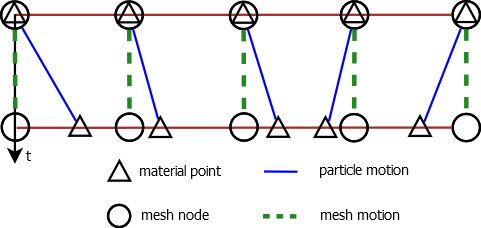
\includegraphics[width=0.8\textwidth]{images/eulerian}
	\caption{Eulerian perspective}
	\label{fig:eulerian}
\end{figure}

A computational mesh can be interpreted as a number of observers distributed across the domain of interest and connected to each other in order to form a a grid with nodes. If the particles of the domain move, a purely euclidean mesh does not move and the position other nodes remain fixed at any instance of time \cite{Cheng2006SlidingFL}. 
This behavior is represented in Figure \ref{fig:eulerian} (adapted from \cite{Cheng2006SlidingFL}). The mesh is independent of particles movement, resulting in a convenient choice for ~\ac{CFD} problems, where fluid flows throughout the whole
computational domain. Within this approach, proper mesh refinement is crucial for computational accuracy as it defines to what extent small scale movement can be modeled and resolved \cite{donea2017arbitrary}.

\subsection{Lagrangian perspective}
\label{subsec:lagrange}

A \textit{lagrangian observer} focuses on a single particles and follows it throughout the motion, as depicted in Figure \ref{fig:lagrangian}. Changes in the quantities of interest are observed at different spatial locations. 

\begin{figure}[htbp!]
	\centering
	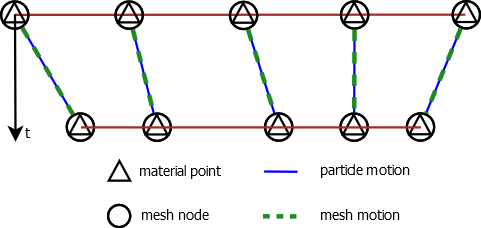
\includegraphics[width=0.8\textwidth]{images/lagrangian}
	\caption{Lagrangian perspective}
	\label{fig:lagrangian}
\end{figure}

The motion of the particle and the other quantities of interest can be described by reference coordinates (or \textit{material coordinates}) in Euclidean space $(X, Y, Z)$, uniquely identifying the observed particle at a reference configuration \cite{XING201957}. Usually $t = 0$ is chosen as reference but this is not mandatory. The Lagrangian observer only registers changes concerning one specific particle as time advances. Thus, quantities of interest can be described as:

\begin{equation}
	\Theta = \hat{\Theta}(X, Y, Z, t)
\end{equation}

In contrast to the Eulerian perspective (Equation \ref{eq:eulerian}), the obtained information is strictly limited to a single material particle (implied by the usage of the capital reference coordinate variables). 
Information about a fixed point in space is not directly available and no convective fluxes appear in a Lagrangian description.

This perspective is again translated into computational meshes: at a reference instance of time, mesh nodes are attached to material particles. As these move, the mesh nodes move with them causing the mesh to deform. Figure \ref{fig:lagrangian} describes the situation. The mesh nodes always coincide with their respective particles.

In this situation large-scale and irregular motions and more importantly deformation lead to distortions of the computational mesh, which yields smaller accuracy in simulations requiring to apply techniques to keep the desired accuracy \cite{lipton2010robustness}.

Lagrangian perspective is the usual method of choice for ~\ac{CSM} simulations.

Eulerian and Lagrangian descriptions are related \cite{bertram2012elasticity}. A mapping between them can described by the \textit{motion} function $\phi$ such that:


\begin{equation}
\vec{x}(t) = \phi(\vec{X}, t)
\label{eq:lag-motion}
\end{equation}

Equation \ref{eq:lag-motion} tells that he Eulerian, spatial position $\vec{x}$ of a particle at time t is the
mapping of the particle at its reference configuration $\vec{X}$: the mapping must be bijective.

\subsection{ALE method}
\label{subsec:ALE}

As outlined above, CSM and CFD problems adopt different perspectives. The ~\ac{ALE} approach, a combination of the two points of view, is used for FSI problems. As the name implies, an ALE observer moves arbitrarily with respect to a specific material particle.
Figure \ref{fig:ale} depicts such a situation.

\begin{figure}[htbp!]
	\centering
	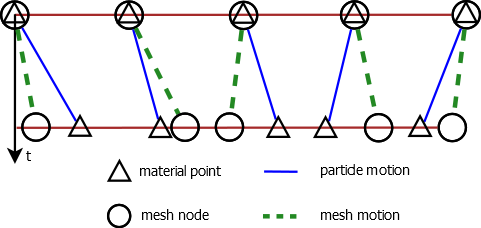
\includegraphics[width=0.8\textwidth]{images/ale}
	\caption{ALE perspective}
	\label{fig:ale}
\end{figure}

When dealing with computational meshes, an ALE mesh is considered as it can move almost arbitrarily with respect to the motion of the underlying particles, as shown in Figure \ref{fig:ale-mesh}.
The only constraint is that node movements should not distort the mesh too much as this leads to computational inaccuracy. Many algorithm exist to implement suitable quality criteria and keep the mesh motion reasonable and to allow the nodes to follow moving particles up to a certain extent \cite{de2007mesh}.

Since the mesh motion and material particle motion are not directly linked, a new unknown is introduced:  the relative movement between the ALE mesh and the material domain. This approach is particularly useful in FSI problems: fluid and solid must follow the moving interface between them for physical reasons.
Since the solid domain is usually described in a Lagrangian perspective, the solid mesh is kept attached to the FSI interface. However, also the fluid domain must deform to avoid formation of gaps between the meshes. Therefore, in ALE methods the fluid mesh nodes at the interface move with it. Fluid mesh nodes follow the fluid particles sticking to the interface (for viscous flows), while the rest of the fluid mesh is allowed to move in such way that mesh distortions are kept minimal, to preserve computational accuracy \cite{ramm1998fluid}.

\begin{figure}[htbp!]
	\centering
	\begin{subfigure}{.5\textwidth}
		\centering
		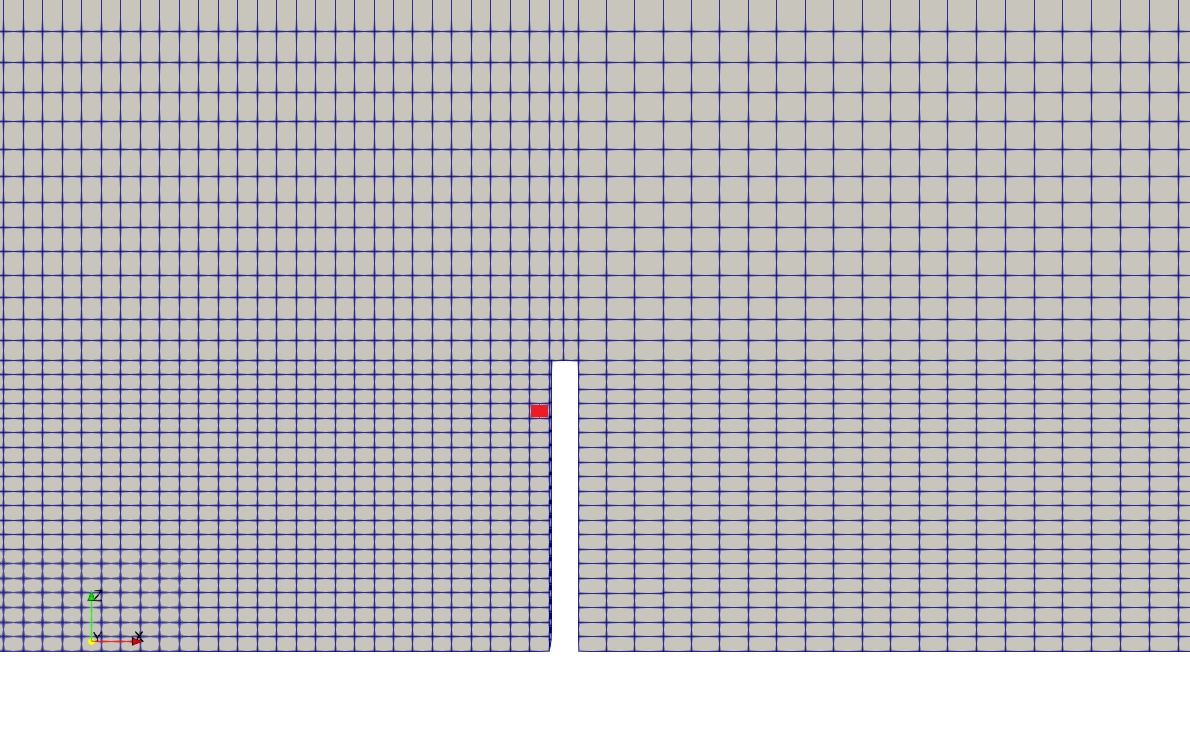
\includegraphics[width=.99\linewidth]{images/undist}
		\caption{undistorted mesh}
		\label{fig:undist}
	\end{subfigure}%
	\begin{subfigure}{.5\textwidth}
		\centering
		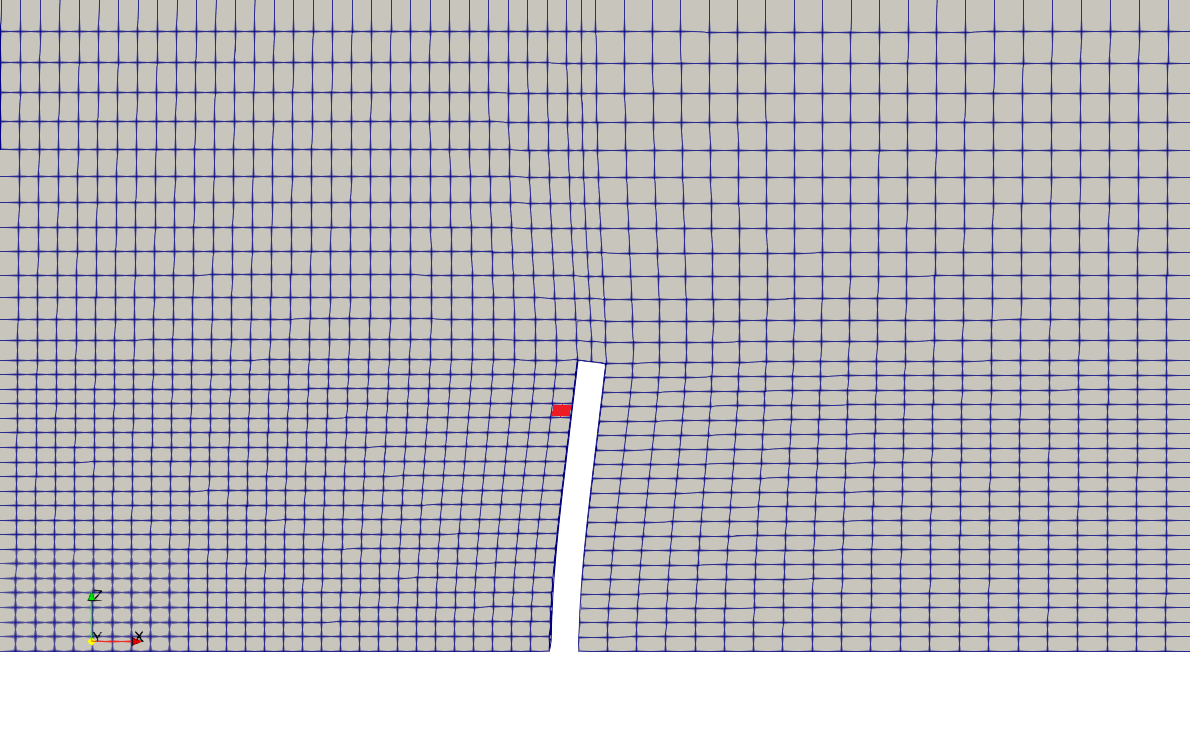
\includegraphics[width=.99\linewidth]{images/dist}
		\caption{distorted mesh}
		\label{fig:dist}
	\end{subfigure}
	\caption{ALE mesh}
	\label{fig:ale-mesh}
\end{figure}

\section{Domains and interface}
\label{sec:models}

Fluid-structure interaction implies that the overall model is determined by models defining the fluid behavior and the solid behavior, briefly described in sections \ref{sec:solid} and \ref{sec:fluid}. A short overview of beam models is given in section \ref{sec:beam} as it is relevant for the model developed in this work.
Finally a formal definition of the interface is given in section \ref{sec:interface}, as it is necessary to define suitable coupling conditions at the common boundary of the solid and the fluid.


\subsection{Fluid domain}
\label{sec:fluid}

An exhaustive description of all possible fluid models is far beyond the scope of this work. A quite general model is the viscous compressible one described by the ~\ac{NSE}. 

\begin{subequations}
\begin{eqnarray}
	\label{eq:cont}
	\frac{\partial{\rho}}{\partial{t}} + \nabla \cdot \left(\rho \vec{v}\right) &=&  0 \\	
	\label{eq:mom-cons} 
	\frac{\partial }{\partial t}\left( \rho \vec{v} \right) + \nabla \cdot \left( \rho \vec{v} \otimes \vec{v} \right) +\nabla p - \nabla \cdot \mathbf{\tau} - \rho \vec{g} &=& 0 \\
	\label{eq:energy-cons}
	\frac{\partial }{\partial t}\left( \rho e_0  \right) + \nabla \cdot \left( \rho e_0 \vec{v} \right) + \nabla \cdot \left( \vec{v}p + \vec{q} -\vec{v} \cdot \bm{\tau} \right) - \vec{v} \cdot \rho \vec{g} &=& 0
\end{eqnarray}
\end{subequations}

where:
\begin{itemize}
	\item $\rho$ denotes density
	\item $\vec{v}$ is flow velocity in all dimensions
	\item \textit{p} denotes pressure
	\item $\bm{\tau}$ is the viscous stress tensor
	\item $\vec{g}$ represents the sum of all body forces
	\item $e_0$ is the total energy per unit mass
	\item $\vec{q}$ is the heat flux by conduction
\end{itemize}

They consist in the mass conservation equation (\ref{eq:cont}), the conservation of momentum equation (\ref{eq:mom-cons}) and the energy conservation equation (\ref{eq:energy-cons}). For a Newtonian fluid, the viscous stress tensor is given by:

\begin{equation}
	\label{eq:tau}
	\bm{\tau} = -\frac{2}{3}\mu \left( \nabla \cdot \vec{v} \right) I +2\mu S
\end{equation}

with $\mu$ being the dynamic viscosity and \textit{S} the rate of deformation tensor (i.e. the symmetric part of the velocity gradient $\nabla \vec{v}$):

\begin{equation}
	\label{eq:def_tens}
	\mathbf{S} = \frac{1}{2} \left( \nabla \vec{v} + \nabla \vec{v}^T \right)
\end{equation}

A detailed derivation of such equations and the theory beyond can be found for example in  \cite{quartapelle2013fluidodinamicaI} and \cite{quartapelle2013fluidodinamicaC} or in \cite{pope2001turbulent}. 

The set of equations above, even with a Newtonian fluid model, lack some other information in order to form a closed set of ~\ac{PDE}. A conductive heat flux model is needed  (e.g. Fourier’s Law), the caloric and thermodynamic equations of state have to be chosen, a proper turbulence model if needed (see \cite{pope2001turbulent}) and finally, the appropriate initial and boundary conditions for the problem \cite{galdi2011introduction} must be defined.

Simplifications can be done to obtain less sophisticated models such as: adiabatic, inviscid, incompressible, and many others. Dimensional Analysis is a powerful tool to determine to what extent some reduced models are meaningful, and it is widely used in fluid dynamics, as described in section \ref{sec:dimensional}. Most CFD software codes allow to set up simulations with the most suitable model which can be coupled with a solid model to build a FSI problem. Some further details are given in section \ref{sec:monolithic}. 


\subsection{Solid domain}
\label{sec:solid}

In solid mechanics, particles do not travel as much as they do in fluid dynamic problems, as described in \ref{subsec:lagrange}. For this reason, a Lagrangian perspective is generally used.  

The  de-Saint Venant-Kirchhoff model \cite{ogden1997non} is very commonly used when describing the movement of a solid: it is also often used in FSI problems ad it is capable of handling large deformation. The material is considered:

\begin{itemize}
	\item \textit{homogeneous}: the material properties do not depend on the position of the particle
	\item \textit{linear elastic}: the stress-strain relationship is linear
	\item \textit{isotropic}: the stress-strain relationship is independent from the direction of the load
\end{itemize}

A general expression of the dynamic equation can be derived from the ~\ac{VWP} applied to an arbitrary control volume: 

\begin{equation}
	\label{eq:mech}
	\frac{\partial^2 \vec{u} }{\partial t^2} = \nabla \cdot \mathbf{T} + \rho \vec{f}
\end{equation}

In equation \ref{eq:mech}:

\begin{itemize}
	\item $\rho$: is the material density
	\item $\vec{u}$: is the particle displacement
	\item $\mathbf{T}$: is the \textit{second Piola-Kirchhoff} stress tensor
	\item $\vec{f}$: is the sum of body forces
\end{itemize}


In order to close the dynamic equation, a constitutive law which must be considered to relate stress and strain:

\begin{equation}
	\mathbf{T} = \lambda \mathbf{I} \mathrm{tr}\left[ \bm{\varepsilon_G}  \right]  + 2\mu \bm{\varepsilon_G}
\end{equation}

where $\bm{\varepsilon_G}$ is the Green-Lagrange strain tensor:

\begin{equation}
	\bm{\varepsilon_G} = \frac{1}{2}\left( \mathbf{F}^T \mathbf{F}-\mathbf{I}  \right)
\end{equation}

and $\mathbf{F}$ is the deformation gradient. $\lambda$ and $\mu$ are material properties and are named Lamé constants. These relate to the Young modulus \textit{E} and the Poisson ratio $\nu$ which are more commonly used in practice. The relationship among the various parameters is the following:


\begin{eqnarray}
	E &=& \frac{\mu(3\lambda+2\mu)}{\lambda + \mu} \\
	\nu &=& \frac{\lambda}{2(\lambda + \mu)}
\end{eqnarray}

The set of parameters $\left(E, \nu\right)$ or $\left(\lambda, \mu \right)$, together with the density $\rho$ fully define the material, under the assumptions of linear elasticity, isotropy and homogeneity.

The set of PDEs is completed when suitable initial and boundary conditions are defined.

\subsection{Models with reduced dimensionality: beams}
\label{sec:beam}

The equations introduced in section \ref{sec:solid} may be a tough task to solve even of the case of isotropic hyperelasticity, when considering a 3-D domain. Even with today's computers and using finite elements techniques, it is not always feasible or convenient to treat a solid as a three-dimensional continuum. Body with particular geometric features can be seen as lower dimension bodies, with respect to the governing equations \cite{hjelmstad2007fundamentals}. Such bodies are called \textit{beams} (one dimension) , \textit{plates} or \textit{shells} (two dimensions).

The \textit{beam} model splits the description of the geometry into two subproblems:
\begin{enumerate}
	\item a beam is defined by its \textit{reference line} and the movement (displacement and rotation) of the solid is completely defined by it (see Figure \ref{fig:beam-model}),
	\item the beam \textit{cross section} is considered as a whole, its movement depends on the movement of the reference line, stresses are generalized into \textit{resultants} (axial, bending, shear, torsional) which represent the aggregate effect of all of the stresses acting on the cross section. The constitutive properties of the section (axial, shear, torsion and bending stiffness) allow to relate stresses and deformations (by means of VWP) and close the problem.
\end{enumerate}


\begin{figure}[htbp!]
	\centering
	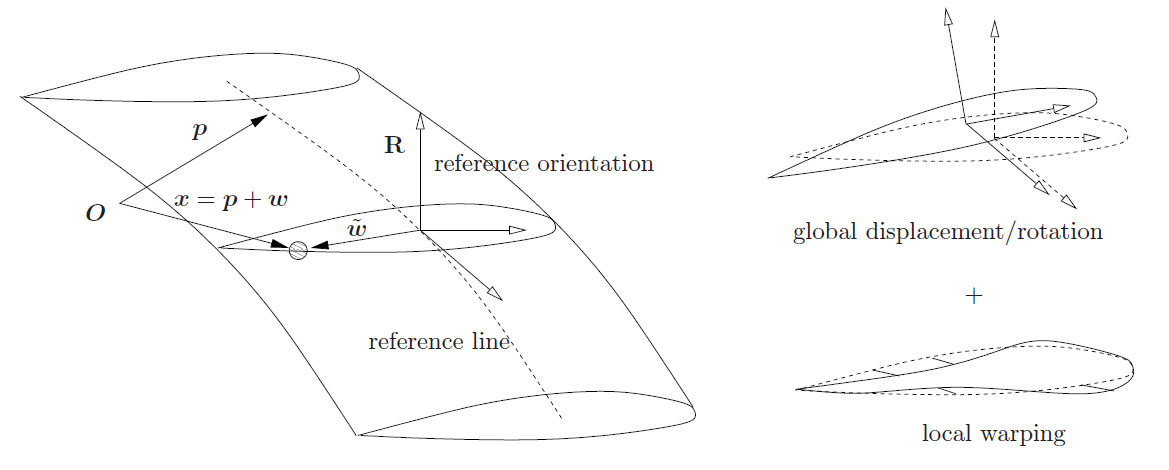
\includegraphics[width=0.8\textwidth]{images/beam}
	\caption{beam model, taken from \cite{ghiringhelli2008integrated}}
	\label{fig:beam-model}
\end{figure}


The beam model can be used to build elements of a ~\ac{FEM}. For example, the beam element can be modeled by means of a Finite Volume approach, as described in \cite{ghiringhelli2000multibody}, which computes the internal forces as functions of the straining of the reference line and orientation at selected points along the line itself, called evaluation points.

\hl{This approach is particularly interesting for FSI problems in which slender structures are involved. A mapping is needed between the fluid-solid interface and the reference line movement, which will be described in.}


\subsection{Interface and interaction}
\label{sec:interface}

Since FSI problems are centered on the interaction of the fluid and solid domain, their common interface needs to be described properly. A simple representation of the situation at the so called \textit{wet surface} is shown in Figure \ref{fig:interface}. Quantities related to the solid use S subscript, while fluid domain and the interface are labeled with F and FS, respectively. 

\begin{figure}[htbp!]
	\centering
	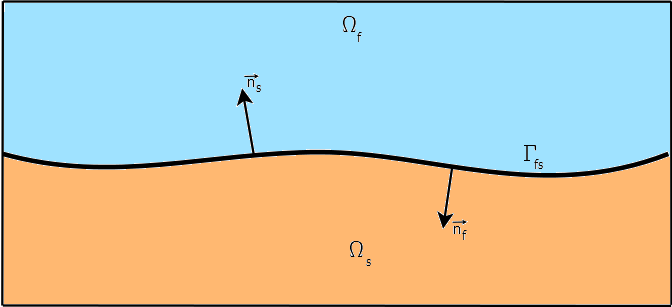
\includegraphics[width=0.8\textwidth]{images/interface}
	\caption{fluid solid interface}
	\label{fig:interface}
\end{figure}

In order to have a physically correct behavior, some conditions have to be met \cite{hou2012numerical}:

\begin{itemize}
	\item solid and fluid domains should not overlap nor separate,
	\item for a viscous fluid model, the flow velocity at the interface must equal the boundary velocity (\textit{no-slip} condition),
	\item for an inviscid fluid model, only velocity components normal to the wet surface have to be equal to the structural 	velocity as the fluid may slip freely in tangential direction at any boundary,
	\item forces exchanged at the interface must at equilibrium.
\end{itemize}

The first conditions result in the \textit{kinematical requirement} that the displacements of fluid and solid domains, as well as their respective velocities have to be equal at the wet surface (denoted by $\Gamma_{FS}$): 

\begin{eqnarray}
 \Delta\vec{x}_F &=& \vec{u}_S \\
 \vec{v}_F &=& \frac{\partial \vec{u}_S}{\partial t}
\end{eqnarray}

The last condition results in the equilibrium requirement. Force vectors are computed from the stresses at the interface and the outward normal vectors of fluid and solid domain, respectively. They have to be equal and opposite leading to the dynamic coupling condition:

\begin{equation}
\bm{\sigma_F} \cdot \vec{n}_F + \bm{\sigma_S} \cdot \vec{n}_F = 0
\end{equation}

$\bm{\sigma} \in \mathbb{R}^{3 \times 3}$ represents the stress tensor (note that for the fluid it comprises pressure and viscous stresses), while $\vec{n} \in \mathbb{R}$ is the outward normal unit vector.


\section{Classification of FSI problems}
\label{sec:classification}
you have been interested in the effect of boundary conditions on the flow. For instance, here is the effect of a cylinder that deviates a uniform flow. In fluid mechanics, we consider solids as boundary conditions only,
and not in terms of what they are made of.
In solid mechanics, we usually consider fluids just as the cause of a loading at the boundary, a force type boundary condition. These two approaches are very useful, and I extensively used in engineering. For instance, in civil engineering you may find engineers that compute wind loads on a bridge. And then send them to other engineers that will check that this is acceptable in terms of the solid mechanics of the bridge. This is often quite sufficient.
We mean situations where you cannot solve these two problems independently.
Here schematically, the cylinder is deformed by the flow, which itself is modified by the deformation of the cylinder. This is coupled fluid and solid mechanics. Now, when you think of it, this question of coupling of models is actually quite fundamental.

First, find a way to classify all these couplings. Why? Because the variety seems so large that it does not seem feasible to find a model that is applicable to all of them. The second objective, once we have classified them is to try and build relevant models for these classes.

So when you want to go from considering dimensional quantities to dimensionless ones, what can you do?
There is a rather general theorem called the Pi Theorem or the Vaschy-Buckingham Theorem, which tells you how many dimensionless quantities you need to look for.
This theorem states that the number of dimensionless quantities, P, is equal to that of the dimensional ones, N, minus R
What is R? It is the rank of the matrix of dimension exponents. This matrix is formed by the columns of the dimension exponents of all variables, as you can see here. Remember that the rank of a matrix is a number of independent lines or columns that you can find. Let us give an example


\subsection{Dimensional analysis}
\label{sec:dimensional}
CFR w1-2

we need to classify all these cases of mechanical coupling between fluids and solids. 
The tool we shall use is called Dimensional Analysis.
It is dimensionless in the sense that we do not need any scale of unit to express it. It is just a number.
Here, let us just take as a principle that a physical law should only relate dimensionless quantities.
There is a rather general
theorem called the Pi Theorem or the Vaschy-Buckingham Theorem, which tells you how many dimensionless
quantities you need to look for. This theorem states that the number
of dimensionless quantities, P, is equal to that of
the dimensional ones, N, minus R. What is R? It is the rank of the matrix
of dimension exponents. This matrix is formed by the columns of
the dimension exponents of all variables, as you can see here.
Let us consider, schematically,
the fluid here in blue and a solid in red. To make things simpler, we assume that
they stand in separate domain of space and that there is no mass
transfer between them. As for the case of drag on a sphere,
we now need to specify what quantities we want to use to define
our problem and what we are looking for. First, the fluid on the left. Let us say that we're looking for
the local velocity U in relation to the coordinate of the point
we consider X and the time T. This is also going to depend on
the viscosity of the fluid, mu, The density of the fluid rho and
the gravity, G. Also the result is going to be different
if I change the size of the domain. So I say the result depends on the size L. Of course, this velocity is also going to
depend on some boundary condition. For instance, an upstream flow
velocity that I call U naught. This is the list of quantities I'm
considering in a given problem in the fluid. Second, the solid on the right. We might want to know the displacement,
csi, at a position X, at a time T. It may depend on E,
the stiffness of the solid, (I shall come back to this later) on it's density, rhoS and on gravity G. Again, it will also depend on the size. And there is somewhere the magnitude of this displacement that is set,
say cdi naught. As you can see here,
I'm quite general in stating what the problem is. Still by stating that this is
the list of quantities that I want to relate by my physical law,
I'm not that general. For instance,
I've excluded the temperature. But we have to choose what is the kind of
problems that we want to consider. And this is already quite general.

\subsection{Dimensional analisys in fluid domain}
\label{key}
CFR w1-3

We are going to start by
something very simple. Doing dimensional analysis separately
in the fluid and in the solid. Imagine now that what
happens in one domain is totally independent of
what happens in the other. For instance, in the fluid. This is what you have
done in fluid mechanics when you have ignored all possible
influence of what happened inside a solid that bounds the fluid. So, we assume that there exist
a physical low that relates the fluid velocity with all the other
parameters, namely X, T and so on. This means that the flow is not going to
depend on the deformation of the solid, because the stiffness E  for instance,
is not included in there. This is pure fluid mechanics. Let us do the dimensional
analysis of this. Here is a law F between
the dimensional variables. There are eight. To use pi theorem, I need to build
the matrix of dimension exponents. Here it is. X is the coordinate, so it is a length. T is a time. U is a  length per time and so on. As soon as you can put some
units on these quantities, you can write the dimension exponents. Now, what is a rank of this matrix? We can find three independent vectors. For instance, here. And certainly no more than three
because the dimension is three. So the rank is all equal to three. I can conclude that we
should be looking for 8 minus 3 equals 5 dimensionless parameters. So, let us write the law
we are looking for in the form of one depending on
only five dimensionless parameters. What are these dimensionless parameters? We know that we should find
five independent ones. I can easily start by defining a dimensional
velocity by diving U by U naught. Both are velocities. So the ratio is dimensionless. Second, X divided by L. Third, something I shall
explain in a moment. Then, of course, the Reynolds
number that combines these four. What else? I haven't used the gravity G so far. So let us use it in
a dimensionless number. Here is what is usually called the Froude
number combining U naught, G and L. These five members are dimensionless and
they are independent. You cannot get one by
a combination of the others. Let us go back to the ratio
U naught T over L. As all dimensionless quantity,
this one can be understood as the ratio of two dimensional quantities,
two lengths, two times. I can write this one as T over T fluid
where T Fluid equals L over U naught. What is L over U naught? It is just the time taken by
a particle of velocity U naught to travel across the distance L. So T fluid is a time scale associated
with convection in the fluid. A very important quantity
that we shall use later. At this stage, we have just written
down the fact that the dimensionless velocity in  the fluid is dependent
on a dimensionless coordinate, a dimensionless  time,
the Reynolds number, the Froude number.

\subsection{Dimensional analysis in solid domain}

Let us now do the same for
the solid alone. Now, we look for a relation between
all quantities on the solid side. F of X,T, csi, E, L, G, tho s chi naught, equals zero. I have singled out the displacement, which is unknown. 
Let us use again the pi theorem. Here is the matrix of
the dimension exponents. We have here, too,  8 quantities, a rank of 3, and so 5 dimensionless parameters to find. What are they? Here is a choice. The dimensionless  displacement where
I've divided csi by the length L. The dimensionless coordinate or
dimensionless time , I will discuss just after, and
two other dimensionless parameters. The first one is the ratio between
the displacement data csi naught  and the length scale of the system. We shall call it the displacement number. When large, the displacements
are large with regard to the size. This is what we call
usually large displacements. The second one combines gravity,
density, length and stiffness and I shall call it
the elastogravity number. When it is large, it means that the deformations induced 
by gravity in the solid are large. For instance, in a jelly cake,
the shape is really effected by gravity. Let us go back now to the dimensional
time that I introduced. I can write this as T over Tsolid,
where Tsolid is L over a velocity C, and this velocity us
square root of E over rho s. What is it? It is actually the scale of elastic
wave velocities inside the solid. So T solid is the time that an elastic
wave takes to go across the solid.


\subsection{Dimensional analysis of coupled problems}

cfr W1-4

We are now ready to undertake
the dimensional analysis of a fully coupled fluid and solid interaction problem. We have done the case of the fluid alone and
the case of the solid alone We're going to use exactly the same
method but considering the fluid and the solid, simultaneously. We are back to our full list of
parameters that define the problem. Let us discuss a bit what
these quantities are. Some of them are only defined on
the fluid side, or on the solid side. This is, for instance, the case of
the viscosity mu in the fluid or the stiffness E in the solid. Others are common to both domains such as
the gravity g or the scale of lengths L. What about our variables of interest, those that we want to
relate to the parameters? I mean, the velocity U or
the displacement csi. One of them is defined in the fluid and
the other in the solid. But now, we are going to consider
that they are related  to all the parameters of the problem without separation.

What are these dimensionless quantities
in such of problem that mixes fluid and solid ? Let us try to give a set of eight
independent dimensionless quantities out of the 11 dimensional ones. I'll start with the one I know. U over U naught, x over L, U naught t over L, the Reynolds number and the Froude  number. That makes five. Now, I  can also use the ones I
know from the solid side, combining the three quantities in a solid,
and that gives us the displacement number,
csi naught  over L, and the elastogravity   number, G. That makes 5 + 2 equals 7. But from the pi theorem I know I should
use eight dimensionless quantities. 

It necessarily mixes things from
the fluid and the solid side otherwise I would have found
it before when doing the uncoupled case. So what is it? What can we imagine as the dimensionless
quantity combining fluid and solid dimensional once.

\subsubsection{Mass number}

 The simplest one is the ratio
of the two densities. Let us call it the Mass Number, M. This seems a very good choice because it
simply tells you that it is different for a solid to interact with air or
with water. In the hard-disk drive example, M is the  order of 1,  air,
over 10 to the 4, metal, and so M is of the order of 10 to the minus 4. Conversely, for the dolphin skin, both media have about the same density,
and M is the order of 1. 

\subsubsection{Reduced velocity}

Here is another possible choice,
the reduced velocity. It is the ratio between our free velocity,
U naught, and the velocity of elastic waves in a solid, c. This also seems a good idea
because it contains information on the way the two dynamics are related. It would be quite different between
two examples I considered before. The inflatable dam and the dolphin's skin. [MUSIC] As possible new dimensionless parameters I
have proposed the ratio of two densities, that was the mass number and the ratio of
two velocities, that was the reduced  velocity.

\subsubsection{Cauchy number}

 I can also imagine something
combining stresses or stiffnes. This here is the Cauchy number. What does it mean? It is the ratio between the fluid loading
quantified by the dynamic pressure over a  unit square and
the stiffness of the solid E. 
The higher it is, the more the solid
is elastically deformed by the flow.


 These three are actually the most
important ones, and are used a lot. Which one should you choose for
your problem? Well as I said before, there is no
good choice of dimensionless numbers. But there are efficient choices, that would be more helpful
in solving a given problem. 



Figure~\ref{fig:first_figure}.
\begin{figure}[htbp!]
\centering

\includegraphics[height=0.24\textheight]{images/logo_poli}
\caption{First Figure}
\label{fig:first_figure}
\end{figure}
\\
